\part{GIS interface} \label{part:gis}
\chapter{Previous concepts}
\label{ch:gis:prev}
    In order to develop a usable interface, we must rely on a map based representation that works with geographic information. Therefore, in this chapter we shall introduce the basic concepts of \gls{gis} in order to provide a context for this part of our contribution.
    
    While there exist several complementary definitions for \gls{gis} in the literature, from the point of view of the current work we will regard a \gls{gis} as an application designed to assist a decision making process related to spatial or geographical information \cite{harmon2003design,longley2015geographic}.
    
    BRIEF OUTLINE.
    
    \section{Spatial information features}
    One of the main challenges in \gls{gis} is the treatment of spatial information, which presents some distinctive features that make it more complicated to store, manage and visualize than the kinds managed by traditional information systems (e.g. an accounting database). We consider that the most significative features of spatial information are:
    
    \begin{itemize}
        \item \textbf{Two alternative conceptual interpretations.} Geographical information may be regarded on a conceptual level from three different perspectives: as geographical objects, as geographical fields or as topological networks. This division on an abstract level will also propagate to the more concrete levels.
        
        \item \textbf{Multiple possible logical models.} The complexity of geographical information makes it so several possible and valid representations can exist for the same geographical phenomenon, each with its advantages or disadvantages depending on the context.
        
        \item \textbf{Data types and specific operations.} Due to the three possible conceptual interpretations and the multiple possible logical models, there are numerous possible datatype sets. Moreover, many different operations that may be defined over these datatypes, and there is no standard for a minimum amount of operations that may be used to define every other operation.
        
        \item \textbf{Complex and varied methods of analysis.} Depending on the field of application that the \gls{gis} is used on, there may exist a great variety of techniques to analyze geographical information that are expected to be included in the \gls{gis}.
        
        \item \textbf{Large datasets.} Geographical information can be quite voluminous, both in the complexity of every element as in the number of elements that must be stored. As a result, the structures used to store this information have to be specific.
        
        \item \textbf{Slow transactions.} The complexity of geographical information can make updating times significantly slow, which in turn can make long locking times on the stored elements. A \gls{gis} must consider updating mechanisms, since its information is naturally dynamic.
        
        \item \textbf{Spatial indexing}. Due to the large size of the datasets, combined with the spatial features (i.e. number of dimensions, space boundaries, etc\dots), the indexing structures that are used to provide an efficient access method to the stored information are particular to a specific use case.
        
        \item \textbf{Implicit hierarchy.} Unlike traditional information, geographical information is always visualized over a bounded space (the map). Because of this, the visualization scale acquires a main role in the presentation of the information and also determines an implicit hierarchy, as it is not possible to display all the information at the same time.
        
        \item \textbf{Special visualization techniques.} A usable interface to visualize geographical information must include commonly expected features, such as interactive controls, a layer abstraction and an acceptable performance to be considered responsive.
    \end{itemize}
    
    \section{Conceptual models}
    \label{gis:concept}
    A first step to define a conceptual model for geographical information is to define the geographic space. To achieve that, we need a mathematical definition of space and to define a \gls{crs}.
    
    \subsection{Coordinate Reference Systems}
    In order to represent a spatial element, we need to define a \gls{crs}, will depend on our mathematical definition of space. One common coordinate system is the Cartesian one, based on an Euclidean space, a plane over which bidimensional objects may be represented. This system, however, is insufficient for broad areas of the Earth's surface, where the curvature of the Earth must be taken into account. To address these cases, the geometry of the planet is often approximated with a spheroid or an ellipsoid, over which spherical coordinates (latitude and longitude) are used instead of Cartesian ones. Currently, the most popular coordinate system is based on the \textbf{WGS84} ellipsoid,\footnote{\url{https://epsg.io/4326}} used for the GPS navigation.
    
    Once the definition of space has been established, we need to choose a coordinate system and define how it will reference the space (origin of coordinates, orientation and scale). Depending on the application, we can directly use the spherical coordinated defined by the ellipsoid or project these coordinates into an Euclidean space. The most common projection to work with relatively small areas of the Earth's surface is the \gls{utm}, which divides the chosen ellipsoid into 60 zones, each one of them spanning 6 degrees of longitude. Within each zone, it is possible to project the curved surface into a plane with minimal precision loss, thus allowing to reference coordinates in a Cartesian system, with a scale of meters, where the first component is the Easting from the central meridian (plus an offset of 500.000 meters to avoid dealing with negative numbers) and the second component is the Northing from the intersection between the central meridian and the Equator.
    
    \begin{example}
    Using a \gls{crs} defined by the WGS84 ellipsoid, the building of the Faculty of Informatics of the Universidade da Coru\~na is located at the coordinates (43.332709,-8.410517).
    Another possible \gls{crs} can be defined by projecting the WGS84 ellipsoid using \gls{utm}, which would place the longitude of the building (-8.410517) into the zone 29, with the coordinates (547788, 4797931). This projection may also be used with a different ellipsoid, yielding a different \gls{crs} with some other coordinates.
    \qed
    \end{example}
    
    \subsection{Abstractions for geographical information}
    Once the \gls{crs} is defined, we must define the abstractions that will allow us to represent geographical information, which can be considered from three alternative perspectives: as geographical objects, as geographical fields or as topological networks.
    
    Geographical objects are subsets of space that are used to represent the position or extension of spatial entities. The surface of a road or the position of a store are examples of geographical objects. Figure~\ref{fig:gis:concept} (left) shows an example of geographical objects on a map.
    
    \begin{figure}[ht]
		\begin{center}
			{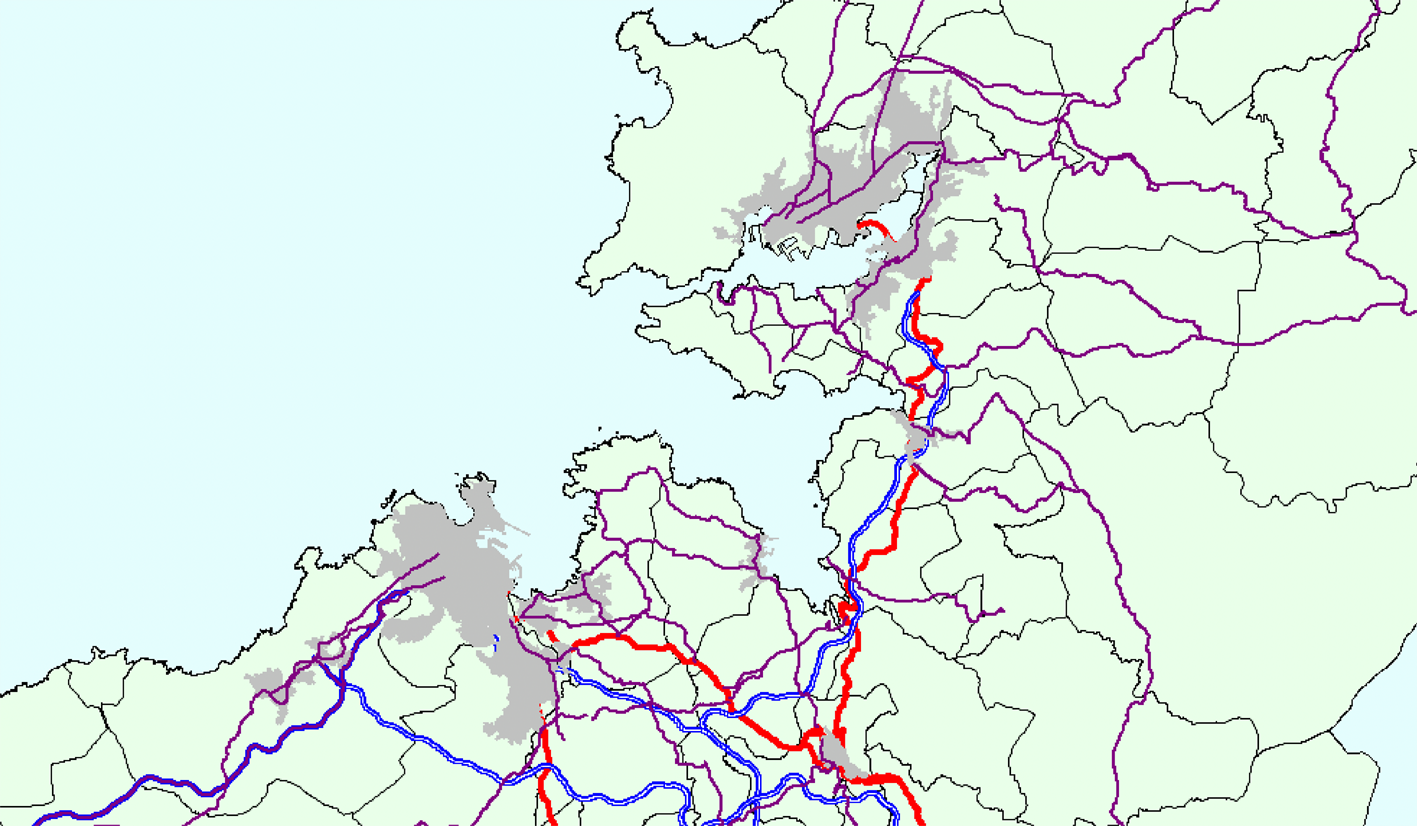
\includegraphics[width=0.45\textwidth]{figures/geo_object.png}}
			{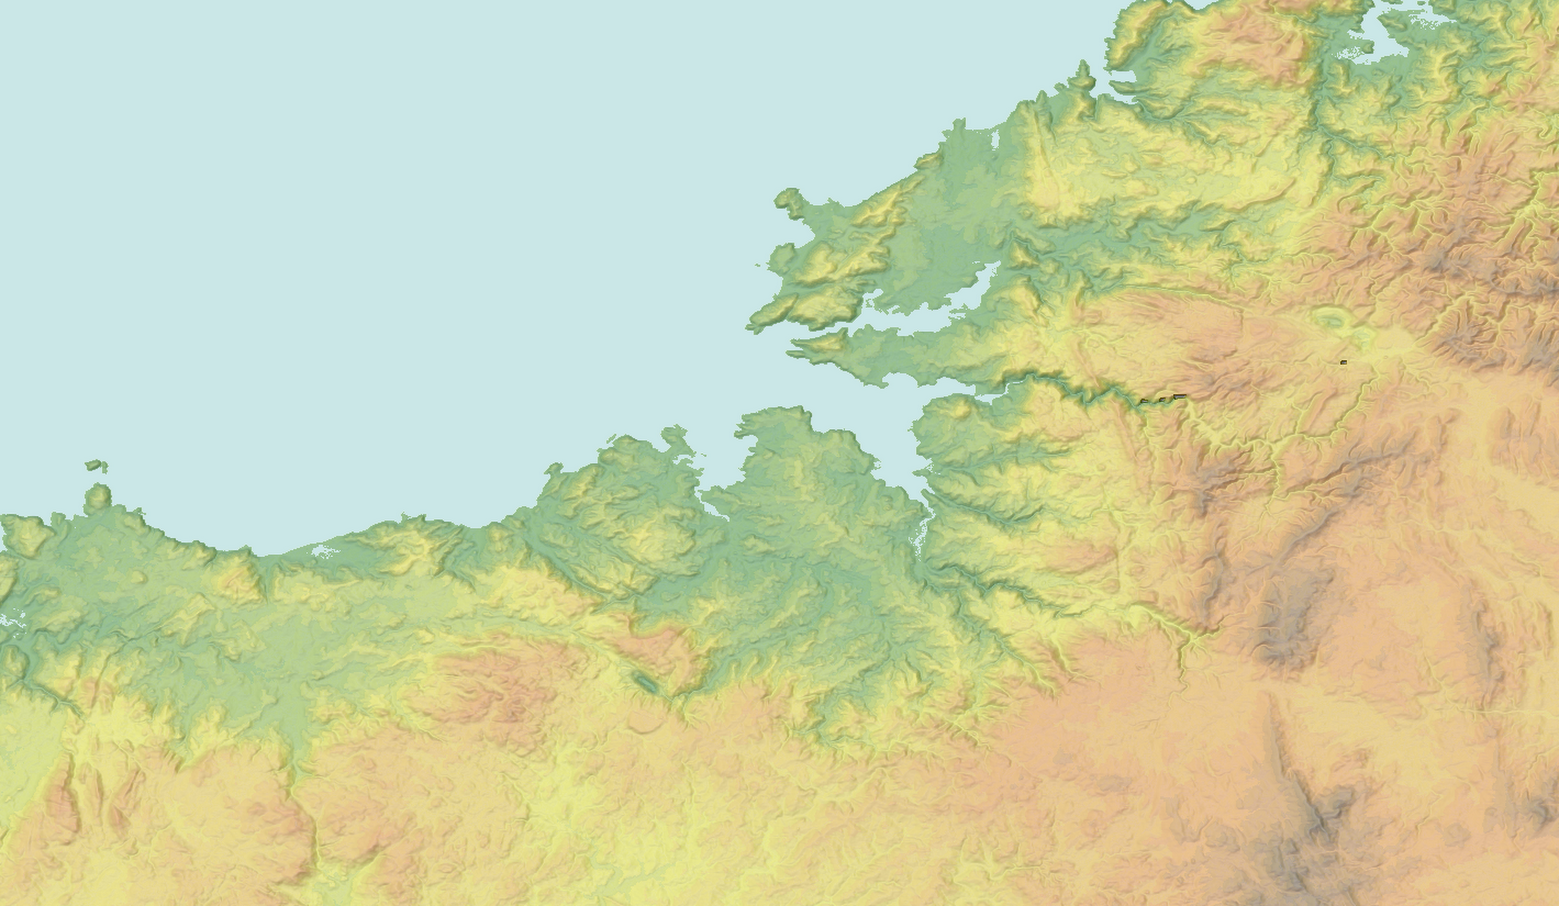
\includegraphics[width=0.45\textwidth]{figures/geo_field.png}}
		\end{center}
		\caption{Two of the possible abstractions for geographical information: geographical objects (left) and geographical fields (right).}
		\label{fig:gis:concept}
	\end{figure}
    
    Note that there can be several valid representations for a geographical object, regardless of its extension in the real world. For instance, a city may be represented as a single position (point) or as a geometric surface, depending on the ultimate requirements of visualization or exploitation.
    
    On the other hand, a geographical field is characterized as a function that associates a value for every point of space. The surface temperature or the slope of the terrain may be considered as geographical fields. An example of a geographical field can be found in Figure~\ref{fig:gis:concept} (right), where an elevation map is shown.
    
    Both abstractions described above (geographical objects and geographical fields) can be alternatively used to represent information of different nature. Commonly, geographical objects are used to analyze man made structures, such as roads, borders or land registry, while geographical fields are more appropriate for natural information collected by sensors, such as meteorological, geological or satellite information. However, this does not mean that, for example, a building cannot be represented as a geographical field that assigns a value of 1 for a coordinate contained within the building and 0 for every other coordinate, although such conceptual definition may be inadequate for many applications.

    There are defined standards for modeling geographical objects, such as ISO 19107, based on primitives objects (points, curves, and surfaces) that may be combined to form more complex types. On the other hand, ISO 19123 is a standard used for modeling geographical fields, which may be discrete (only existing a value for some discrete points in space) or continuous, having a value for any point in space.
    
    As a special case, it is also possible to work with a topological network, where instead of using a coordinate system, we can model our space as a graph. An example of such application may be a road network used for GPS routing, where the movement is restricted by roads instead of a true Euclidean space. While there are also standards for these abstractions, it is more often to use an ad-hoc model based on vertices and edges.
    
    \section{Logical models}
    In the previous Section~\ref{gis:concept}, we have defined conceptual models, that work on an abstract level. However, the abstract models do not regard the limitations of a practical implementation. As such, they may assume that both the memory and arithmetic precision are infinite, and consequently a geographical object is an infinite set of points while a geographical field is a defined function for any point in space. These limitations must be addressed in order to implement a \gls{gis}, and for that purpose we must work with a logical model.
    
    In this section we will present two well known models used to represent geographical information, although we will not cover how the most used operations are implemented using these models or how the precision problems may be addressed. Refer to \cite{xiao2015gis} for a more in-depth coverage on those topics.
    
    \subsection{Vector model}
    This model uses numerical data types (such as integers or floating point representations) to deifne a system of coordinates over which the geographical information is represented using geometric constructions (points, segments, polygons, etc\dots). For each primitive data type defined in the geographical object conceptual model, there is a vector representation.
    
    The most extended vector model is the Simple Feature Specification, defined by the Open Geospatial Consortium (OGS), in which data types are defined to represent simple spatial objects defined in the ISO 19107. The simpler data types are composed to represent more complex ones, as shown in Figure~\ref{fig:gis:sfc}, where a \textit{curve} is approximated as a \textit{LineString}, which is defined as a sequence of \textit{points}, while a \textit{surface} can be a \textit{Polygon} defined with \textit{LinearRings}, which are special cases of \textit{LineStrings} where their last \textit{point} is equal to the first one, thus enclosing a space.
    
    \begin{figure}[ht]
		\begin{center}
			{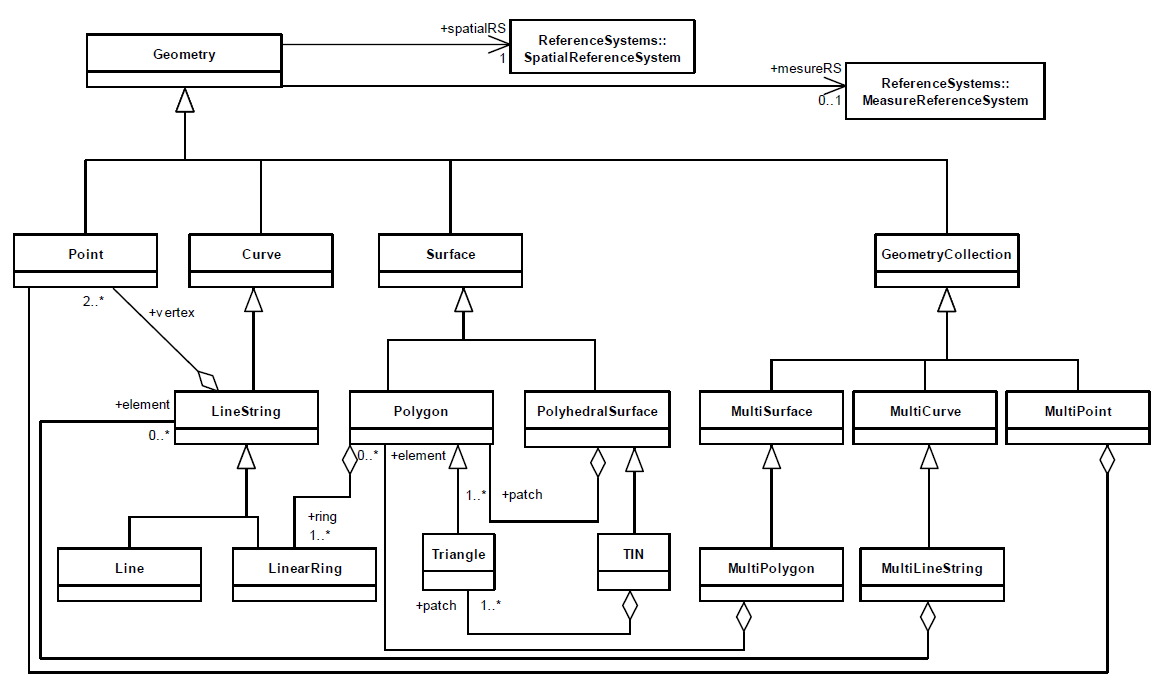
\includegraphics[width=0.98\textwidth]{figures/sfc.png}}
		\end{center}
		\caption{The data types of the Simple Feature Specification by the Open Geospatial Consortium}
		\label{fig:gis:sfc}
	\end{figure}
	
	This composition can be also seen in Figure~\ref{fig:gis:sfcexample}, where six \textit{points} are used to define a \textit{LineString}, while three \textit{LinearRings} are used to define a \textit{polygon}, one for the external borders of the \textit{polygon} while the other two define the internal borders (the {\em holes}).
	
	\begin{figure}[ht]
		\begin{center}
			{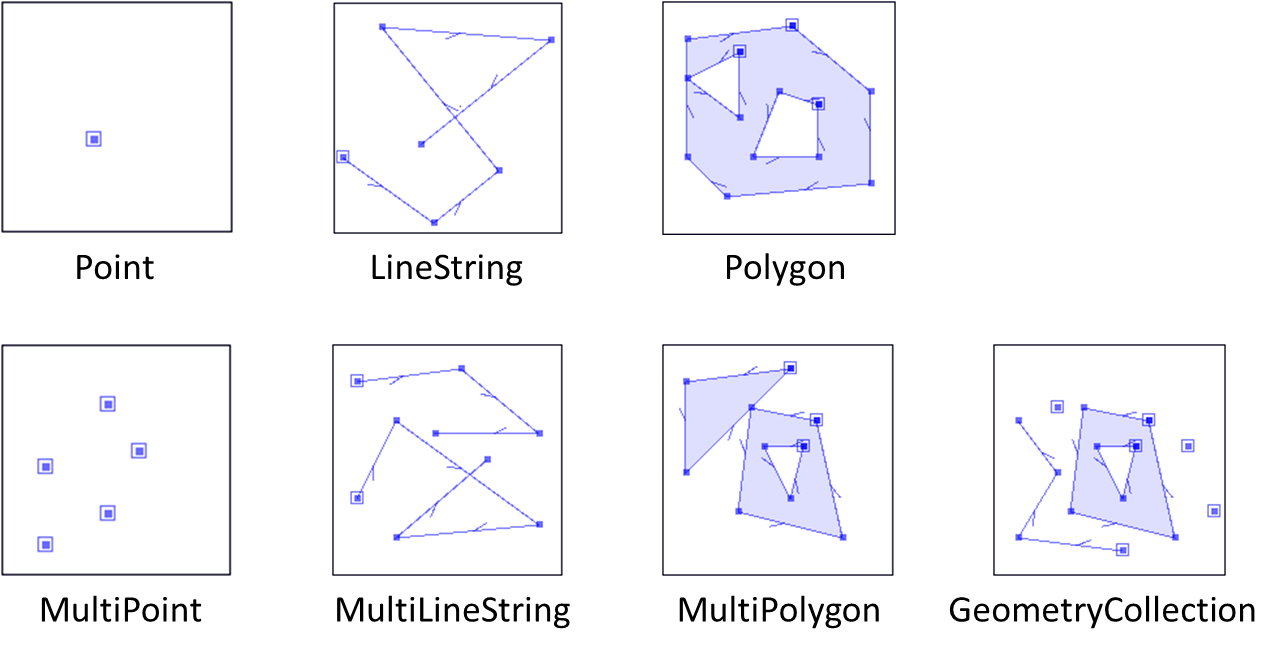
\includegraphics[width=0.8\textwidth]{figures/sfc_example.png}}
		\end{center}
		\caption{Examples of Simple Feature Specification data types.}
		\label{fig:gis:sfcexample}
	\end{figure}
    
    \subsection{Raster model}
    \label{sec:raster}
    The raster model represents the spatial information using a matrix, where every cell stores a value for a portion of the space. The meaning of each value will depend on the particular case. To cite some examples, the value of the a cell may be temperature, pressure, humidity, wind speed or the color of the surface. In order to translate a cell position to coordinates in a \gls{crs} and vice versa, we need six values: the position of the origin of coordinates and how much the height and width of each pixel contribute to the x and y coordinates in the \gls{crs}. Since the raster may be oriented in any angle, a single dimension in the matrix (such as the width) may contribute to both the x and y components in the \gls{crs}.
    
    Rasters are frequently stored within an image format with some additional metadata for the \gls{crs} transformation. An extension of the {\em TIFF} format called {\em GeoTIFF}\footnote{\url{https://www.opengeospatial.org/standards/geotiff}} is one of the most common formats for these purposes, as it allows to define a \gls{crs} and the linear transformation parameters for coordinates. Additionally, it is possible to store several images in a single TIFF file, which is often used to store several levels of detail for the raster, allowing to speed up operations that do not require the highest resolutions.

    \subsection{Comparison of vector and raster models}
    In the previous section we have described two possible logical models to represent geographical information: the vector and raster models. Both models can be used to represent either geographical objects or geographical fields. As previously seen, each model has a different approach to the practical limitations when implementing a conceptual model. In this section we will show how each of the logical models can represent either geographical objects or geographical fields and also make a brief comparison of both models.
    
    In the vector model, geographical objects are represented as a discretization, which may lead to some precission loss in some of the shapes, as seen in Figure~\ref{fig:gis:object} (top). In the other hand, the raster model can represent objects by a process called \textit{rasterization}, where each cell value is assigned to an object identifier, as seen in Figure~\ref{fig:gis:object} (bottom).
    
    \begin{figure}[ht]
		\begin{center}
			{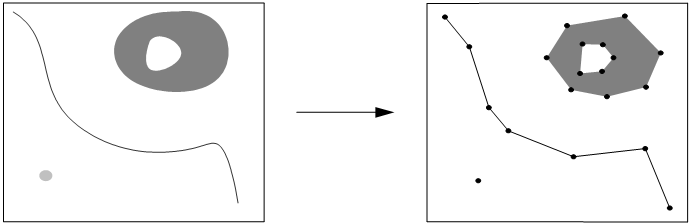
\includegraphics[width=0.8\textwidth]{figures/obj_vector.png}}
			{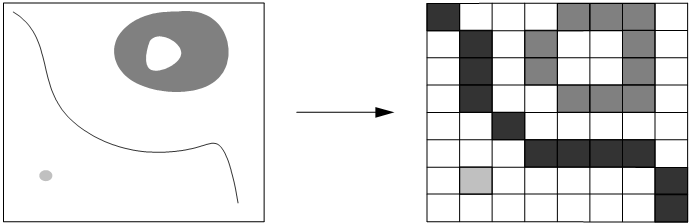
\includegraphics[width=0.8\textwidth]{figures/obj_raster.png}}
		\end{center}
		\caption{Representing geographical objects in the vector (top) and raster (bottom) models.}
		\label{fig:gis:object}
	\end{figure}
	
	Geographical fields are also transformed when they are represented in a logical model. As such, in the vector model, these fields are represented with a polygonization of the function, as shown in Figure~\ref{fig:gis:field} (top), while in the raster model we discretize the function, representing a value only for the cells of the matrix, as done in Figure~\ref{fig:gis:field} (bottom).
    
    \begin{figure}[ht]
		\begin{center}
			{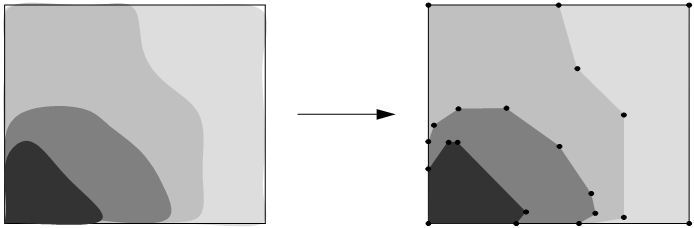
\includegraphics[width=0.8\textwidth]{figures/field_vector.png}}
			{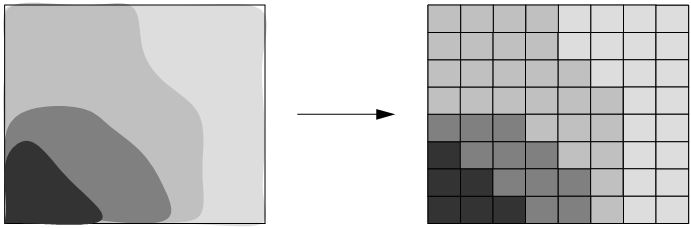
\includegraphics[width=0.8\textwidth]{figures/field_raster.png}}
		\end{center}
		\caption{Representing geographical fields in the vector (top) and raster (bottom) models.}
		\label{fig:gis:field}
	\end{figure}
    
    As both models are interchangeable, the best choice will depend on the specific \gls{gis} application intended. The decision can be influenced by the representation size (vector model is usually more compact), the processing efficiency (raster algorithms are often more efficient and straightforward than the vector ones), expressive capabilities, visualization (the precision of the vector model vs the efficiency of the raster one) or source of the information.
    
    \section{Standards}
    \label{sec:gis:std}
    Over the years, many \gls{gis} standards have been developed and adopted by the community, making it easier to develop and integrate application using multiple data sources. In this section we are only going to cover the standards used by our developed interface.
    
    \subsection{TMS}
    The Open Source Geospatial Foundation defines a standard to generate cartographic images (tiles) called \gls{tms},\footnote{\url{http://wiki.osgeo.org/wiki/Tile_Map_Service_Specification}} which aims to simplify and modernize some aspects of an older standard called \gls{wms}.
    
    A \gls{tms} service returns map parts, called \textit{tiles}, at several levels of zoom with {\em HTTP GET} requests, typically in PNG format, although other formats can be supported. With a special metadata request that returns the definition of the \gls{crs} and the parameters to translate pixel coordinates to \gls{crs} coordinates (discussed in Section~\ref{sec:raster}) at all the supported zoom levels, it is possible to develop a web map application, loading tiles interactively as a user spans and zooms over the map.
    
    It is also possible to integrate \gls{tms} from several sources, as tiles can have transparent background. This could allow, for example, to paint tiles containing only bus lines over tiles showing the streets of a city. Due to its ease of implementation, both server side and for client libraries, this standard has been widely adopted and made available by operators such as OpenStreetMap, Google, Thunderforest and many others.\footnote{\url{https://wiki.openstreetmap.org/wiki/Tile_servers}}
    
    \subsection{GeoJSON}
    While there is a well known web standard for accessing geographical features defined by the Open Geospatial Consortium called \gls{wfs},\footnote{\url{http://www.opengeospatial.org/standards/wfs}} which allows to obtain, among many other kinds of information, the vector representation of the geometry for these geographical features, this standard is often found too complex for the single purpose of transmitting vector geometries.
    
    For this reason, custom \texttt{REST API}s that encode vector geometries in GeoJSON\footnote{\url{https://geojson.org/}} (RFC 7946) have become the most popular way of transmitting this data. This format makes it possible to encode \textit{Points},  \textit{LineStrings}, \textit{Polygons} and their multipart variants in a compact string, while also allowing to attach any arbitrary information (\textit{properties}) to these features in JSON format.
    
    \subsection{GTFS}
    Developed as a standard to represent the schedules of most public transportation systems, \gls{gtfs}\footnote{\url{https://developers.google.com/transit/gtfs/}} was developed by Google and it provides a standard model to specify stops, routers, schedules and other useful information for trip planning that may be associated with a transportation system, as shown in the diagram from Figure~\ref{fig:gis:gtfs}.
    
    \begin{figure}[ht]
		\begin{center}
			{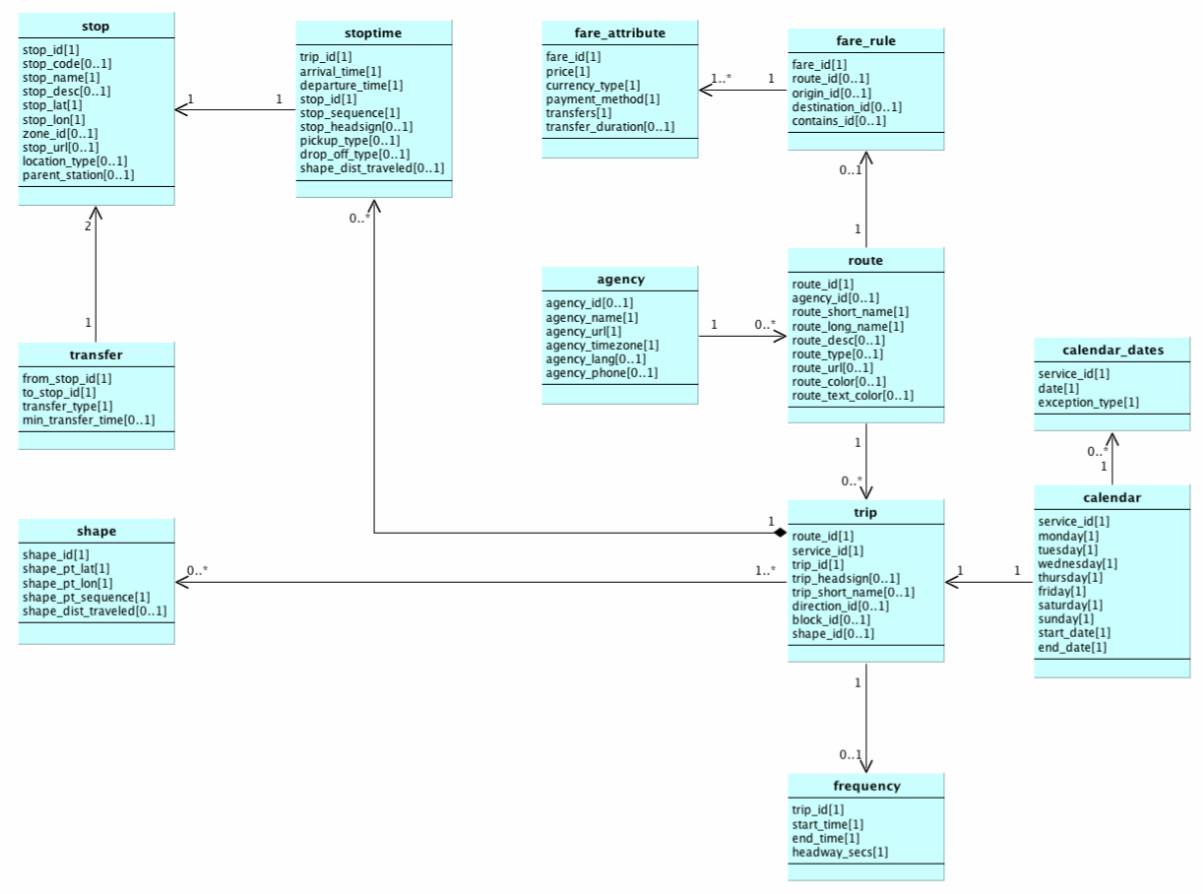
\includegraphics[width=0.95\textwidth]{figures/gtfs.png}}
		\end{center}
		\caption{UML class diagram of the entities specified by \acrshort{gtfs}.}
		\label{fig:gis:gtfs}
	\end{figure}
	
	This has some resemblance to the model we have previously proposed in Figure~\ref{fig:er} from Section~\ref{sec:newctr:desc}, where a \texttt{stop} in \gls{gtfs} corresponds to a \texttt{stop\_place} in our model, \texttt{stoptime} to \texttt{stop\_time}, a \texttt{trip} is similar to a \texttt{journey}, while a \texttt{route} is a \texttt{line}. The largest difference, however, is that we consider that a line (route) is formed by fixed sequence of stops, while in \gls{gtfs} no such restriction exists, and every trip can theoretically have a different sequence of stops.
	
	There are GPS coordinates stored for a stop, and it is also possible to define a \textit{LineString} shape for a trip, which will be referenced by a \texttt{shape\_id} from a shapes definition file. The stop times for a trip are usually defined within the calendar dates, allowing this way to specify a schedule based on the day of the week or have a special consideration for selected days. Outside of the calendar definition, it is still possible to specify an expected frequency that a trip must respect.
    
    \section{GIS interfaces}
	In the previous sections we have discussed how to represent geographical information in conceptual and logical models, as well as what \gls{gis} standards are followed in this work. In this section we will briefly speak about how this geographical information can be presented to the user and visualized in a \gls{gis} interface, as well as introduce a web mapping library called {\em Leaflet} library.\footnote{\url{https://leafletjs.com}}
    
    \subsection{Data visualization}
    The visualization of geographical information is often complex due to the special features of spatial information. In the first place, these features require a different abstraction than the ones used by traditional databases. In the second place, this information usually needs to be transformed with a projection to be able to visualize it on a flat surface. It is also necessary to define a \textit{visualization metaphor} for the user interface: the stored geographical information is presented to the user in several layers.
    
    A layer can be seen as a set of geographical elements that are intended to be visualized with a common style. These layers are later sorted in a stack, to determine which layers are superior or inferior to others. That way, the information of the superior layers is presented over the information of the inferior ones.
    
    This system of layers allows to display a digital map in a similar fashion to a paper map. However, in a \gls{gis} user interface is fundamentally different from a conventional map, as the information is never static. Hence, the interface needs to support interactive operations that can alter this visualization. Among these operations, we would like to mention the following:
    
    \begin{itemize}
        \item Layer management, with the possibility of adding or removing layers, as well as reordering them in the stack.
        \item Scrolling over the map, defining a new point of origin.
        \item Changing the scale of the visualization, increasing or reducing the zoom level.
        \item Invocation of processing operations over the map. These may include, among others, interactive measurements or queries about the visualized elements.
    \end{itemize}
    
    Another important element in this visualization is the context information, which must be included in the user interface in order to understand the displayed information. This context information frequently includes a graphic legend, which allows to interpret and categorize every geographical element. Additionally, the interface must have means to inform the user of the current visualization scale and the center coordinates. Other information may be necessary, such as labels that identify geographical objects or present relevant information.
    
    \subsection{Leaflet}
    Among the several available alternatives to develop a web based map, in this work we are using {\em Leaflet}, which is an open source \texttt{Javascript} library that can be integrated with different data sources and providers to easily develop interactive maps with the standard web technologies (\texttt{HTML}, \texttt{CSS} and \texttt{Javascript}).
    
    It supports both the \gls{tms} and the {\em GeoJSON} standards described in the previous Section~\ref{sec:gis:std}, among others. This combination is often used to display a base map from a tile provider with vector information layers over it obtained in {\em GeoJSON} format.
    
    Although this library is comparatively lacking in features when compared to other well-known alternatives such as Google Maps\footnote{\url{https://developers.google.com/maps/documentation/}} or {\em OpenLayers},\footnote{\url{https://openlayers.org/}} it is frequently preferred due to its usability and smaller size. Due to its broad adoption, open source plugins exist for all the features offered by the other comparable solutions, including support for other data sources (such as \gls{wfs}), advanced features (such as routing) and also small interface tweaks (such as the integration of a context menu).
    

\chapter{GIS interface for public transportation networks}
\label{sec:gis}
	While in the previous part of this work we have presented compact representations that are capable of efficiently handling large collections of trips over both streets and public transportation networks, in order for it to be actually usable by city management and network administrators a front-end interface must be conceived.
	
	In order to facilitate this kind of analysis, we have developed a proof-of-concept map-based interface based on \gls{gis} and web technologies called \textbf{Trippy}, that allows to exploit some of the capabilities of \gls{xctr} to visualize and query transport demand information over a real transportation network. This constitutes a tool is designed to aid the decision-making process for a public transportation company, and can be easily adapter for different networks and use cases.
	
	In this chapter, we will begin by contextualizing the use case in more detail. After that, we provide an overview of our architecture, both from a functional perspective and a technical one. After that, we will present our API for querying the underlying structure, and finally our prototype user interface.
	
	\section{Motivation}
	\label{sec:gis:intro}
    Collecting historic locations and movement patterns is currently a hot topic, as more mobile phone corporations, car companies, and other organizations are trying to get advantage on the market through these modern initiatives. While users are tracked and benefit of their services (avoiding traffic congestion, locating restaurants and monuments, etc. on Google Maps; getting the best route on public transport to go somewhere or getting real-time schedule for a bus/train line, etc) those companies are also obtaining valuable data that can be exploited to obtain a profit or to improve the assignment of their resources (e.g., personalized recommendations and advertising, estimating the number of passengers and consequently the number of trains or buses that are required to support all the passengers that will use a line today, etc).
    
    If we focus in public transport, such as buses or trains, we find that most transport companies have been focused mainly on providing helpful information to their passengers regarding the existing offer, hence providing non only information related to their transport network (e.g. maps with the lines, their schedule, etc.) but also, in many cases, real-time information with the actual position of a vehicle, remaining time to destination, remaining time until next vehicle arrives, etc. 
    However, although there is also an increasing interest on gathering actual information regarding what users demand from the public transport and how they use their services, to the best of our knowledge, there are no final end-user tools that have tackled both the problems of: {\em (i)} effectively handling the huge amount of data that arises when we track all the user's trips (e.g. within a large city) and {\em (ii)} efficiently exploiting the underlying information.
    %Obtaining such  data necessarily required using some technology to track user's movements along the transport network. Currently, it is not uncommon to find cities having a smart card system \cite{smartCards00}, where each user has a personal public transport card with which he or she can pay for trips over several means of transport (bus, subway, etc) and also to switch between them. The use of these smart cards lets the transportation system to know where and when an individual started a trip, which provides valuable information for the administrators of the system. Indeed, the ending stop of a trip can be also estimated from boarding records alone \cite{wang2011review, alsger2016validating}.
    %Several works have also been presented regarding how travelers switch lines or where they finish their trips in order to completely track down any traveler \cite{daniil18,MUNIZAGA2012x}.  This new available information has been exploited in several scopes. For example, to gather the preferences of users on the chosen mean of public transportation to travel through a city \cite{publicTrans17}, to monitor urban traffic \cite{trafficMonit17}, or to study the traffic effects of the congestion charges introduced in some urban areas around the world \cite{congestion15}. However, to the best of our knowledge, there are no final end-user tools that have tackled both the problems of: {\em (i)} effectively handling the huge amount of data that arises when we track all the user's trips (e.g. within a large city) and {\em (ii)} efficiently exploiting the underlying information.
    
    %\ojo{Meter de alguna forma que tantos viajes, puntos de subida etc etc es big data y no hay ninguna olución final implementada ESCALABLE que permita tratar estos datos EN PROFUNDIDAD (HASTA AHORA que nosotros hemos resuelto el  puzzle)}
    
    
    Therefore, we are focusing on a solution to query and visualize historical records of aggregated patterns of movement from the travelers of a transportation network. While there exist popular solutions such as Google Maps to accurately calculate optimal multi-modal routes and even monitor the real time condition of the transportation networks, as indicated above, these systems only manage information about the {\em offer} of the network (such as schedules) and sometimes the real-time {\em demand} (current traffic conditions). In contrast, our approach aims at satisfying query needs about the historical demand over a large collection of past trajectories collected from users.
    
    %As we start handling and storing all those huge amounts of transport information we run into a popular problem nowadays: managing and exploiting big data. This problem has been analyzed  from several perspectives and a significant number of papers about this topic have been presented \cite{bigdataIOT,bigdataBIO}. In the context of public transport the issue is even worse due to the spatio-temporal nature of the knowledge. Spatio-temporal big data is a quite recent research topic that not only needs to deal with how a huge amount of spatial information should be stored and administered \cite{richter12} but also needs to review how this data should be displayed \cite{cortinas18,pelekis11}. Therefore, in this area we have to deal with two important problems: not only processing massive amounts of geographical information efficiently is required, but also developing user-friendly interfaces to access and visualize them are necessary \cite{7363974,LI2016119}.
    
    
    When dealing with vast amounts of historic traveler data, a valid first approach to tackle its analysis is to extend a traditional \gls{dbms} that could both assimilate and handle greater volumes of spatial data. A popular tool that fits in this description would be \textit{postGIS},\footnote{\url{https://postgis.net/}} a spatial extension for the widely adopted relational DBMS \textit{PostgreSQL}. 
    However, these solutions that include spatial indices are not the most adequate for our information needs, that are many times unrelated to a geographic component, but to the network elements and their relationships (``how many travelers started their trip at a stop X using line L to end it at a stop Y within the time frame T?''), while the large sizes of our data collections would force us to use solutions based on secondary memory, considerably affecting the performance of the system.
    
    %\ojo{Deberíamos falar de solucions distribuidas, que usen BD NoSQL,... botar un ollo a isto: \cite{XYGL2018}}
    
    
    
    %Apart from providing an efficient representation for the underlying data, there also exists the need for supporting visualization, exploitation, and management of spatial data by external users. The research in these topics is relatively new, meaning that, to our best knowledge, there does not exist a standard model of representation. Even though normally the users of applications that handle transportation-oriented data have advanced knowledge of geoinformatics, our target is to design a user-friendly interface that would not require of such skills, but only the minimum necessary understanding of the transportation domain.
    
    
    
    %In this work, we focus in the problem of managing data from a public transport system and we present a tool that includes a user-friendly interface to simplify the visualization and exploitation of the underlying data.  Our tool takes advantage of the recent \gls{xctr}\ structure presented in \cite{daniil18} that uses compact data structures to represent the data related to user's trips and efficiently solves some queries on aggregated data. This permitted us not only to save storage space but also boosted query performance when solving some important queries from a public transportation management system. 
    %To the best of our knowledge, it is the first tool that uses a representation of the data based on compact data structures.
    %While there exist other previous works that make use of compact data structures to efficiently index large collections of in-network trajectories \cite{brisaboa2018compact, koide2018cinct,  koide15}, the recent \gls{xctr}\ solution in \cite{daniil18} is novel as it implements a conceptual model that could adapt to any particular transportation system. To decrease the redundancy in the representation of user's trajectories, instead of listing all the stops traversed along a user's trip, \gls{xctr}\ stores only the stops where a user boards a vehicle along a whole trip that chains several lines, and the intermediate stops may be easily deduced from the network representation. 
    
    Given that we are focusing on a tool specifically for public transportation networks, our interface is built over the \gls{xctr} (introduced in Section~\ref{sec:newctr:str:xctr}), which has allowed us to achieve fast response times in our tested use cases. In any case, our proposed tool is flexible enough to allow data to be represented in a more traditional way, such as with a relational \gls{dbms}.
	
	\section{Architecture}
	In this section we discuss the overall architecture of Trippy, our interface based on \gls{xctr}. We start by describing it from the functional perspective, following the data flow from the data sources until the presentation in the user interface. We complement this description with a technical architecture overview, speaking about how the individual components are integrated together and facilitate an understanding of the decisions behind the technological choices.
	
	\subsection{Functional architecture}
	We have designed Trippy to be as flexible as possible, ensuring that it can operate with any network and trip descriptions that can be adapted to the model from Figure~\ref{fig:er}, which is elementary enough to apply to most of the current transportation systems. For an overview of this data flow, refer to the diagram in Figure~\ref{fig:arch:functional}.
	
	\begin{figure}[ht]
		\begin{center}
			{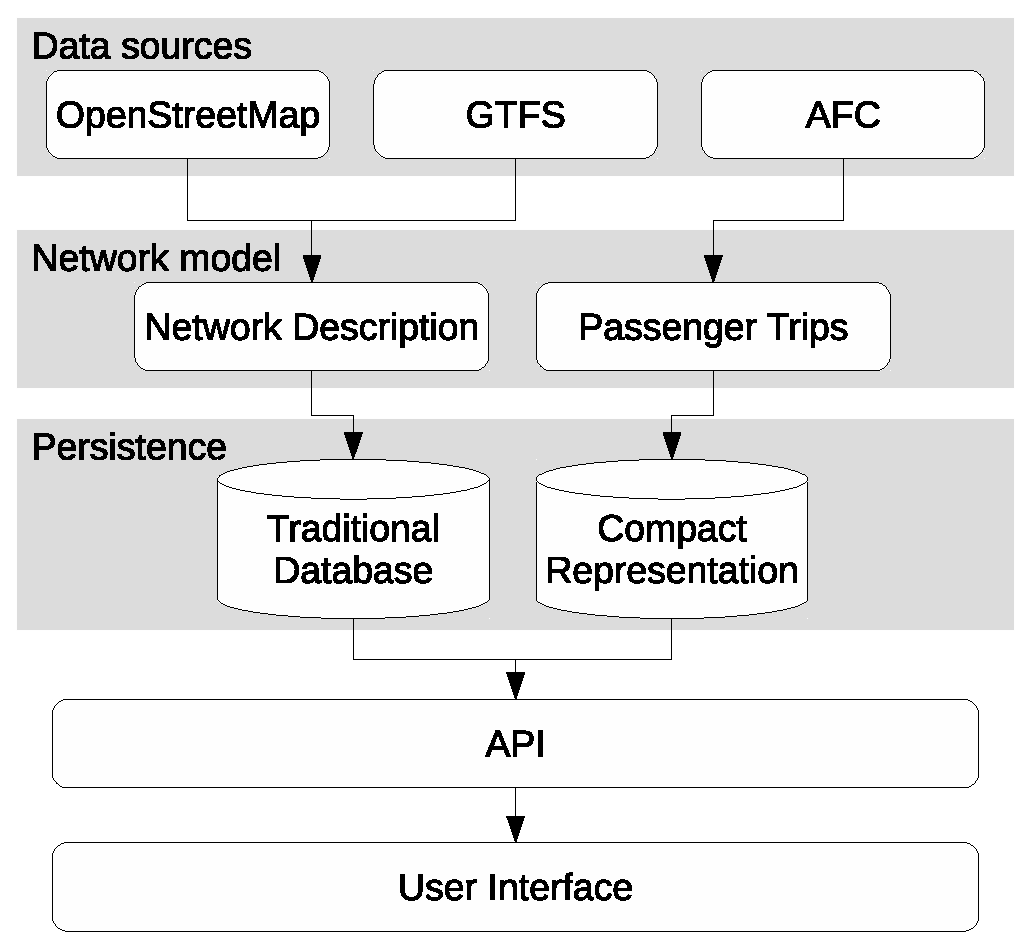
\includegraphics[width=0.75\textwidth]{figures/funcional_trippy.eps}}
		\end{center}
		\caption{Functional architecture of Trippy.}
		\label{fig:arch:functional}
	\end{figure}
	
	Although our system is oblivious to the specific data sources, we have successfully experimented adapting information collected from \gls{gtfs} sources, as well as OpenStreetMap, to obtain a description of a public transportation network. Each different source or format would require a custom conversion to adapt it to our model, which is one of the reasons that we had for standing against overcomplicating our model. As for the passenger trips, they must be described in terms of stages (boarding and alighting pairs) that are related to stops and journeys. The amount of preprocessing needed will depend on the source of the data, as most \gls{afc} systems do not directly record the alightings and the specific journey within the day will have to be estimated based on timestamps.
	
	We have also opted for different persistence options for the network description and the passenger trips, as we are interested in using our \gls{xctr} for the latter, while the former does not pose any technological challenges that would warrant the use of a compact representation.
	
	Finally, these two data repositories are used to feed an API over which requests can be made, which is going to be exploited by the user interface. The specific supported requests are discussed in Section~\ref{sec:api}.
	
	\subsection{Technical architecture}
	We have designed and implemented the infrastructure needed to solve our query needs, which are focused on the usage of network elements, as previously explained in Section~\ref{sec:gis:intro}. 
	%It is also worth highlighting that apart from that main target of Trippy, the second challenge addressed in our system is to efficiently represent massive datasets of trajectories formed by user's trips along a public transportation network. 
	To visualize and query on these network elements, we need to work with a representation of the network itself. Specifically, we represent the model for trips over a public transport network shown in Figure~\ref{fig:er}, extended with spatial attributes (gps coordinates) for the stops and lines. Implementing this model for networks does not pose any challenge, as this information is rather static (it is not expected to grow significantly) and only requires a small amount of space in comparison to passenger trips. Therefore, a \gls{rdbms} representation can be used  to represent the elements of the network. On the other hand, we use our compact representation \gls{xctr} for the trips, that we are going to rely on for most of our queries. The reduced size of this autoindexed representation allows us to keep it in primary memory, making it outperform any traditional indexing alternative that is based on secondary memory.

    The overall technical architecture of our proposal is presented in Figure~\ref{fig:arch:real}. In the bottom part, we can find the backend
    %Before we explain each component in detail, we present a diagram for the overall architecture in Figure~\ref{fig:arch}. It is based on 
    that includes two sources of information: the former one includes the network representation and relies on a small read-only database implemented in SQLite\footnote{\url{https://sqlite.org/index.html}}; the other source includes a \gls{xctr}, for our compact representation of the passenger trips.
	
	\begin{figure}[ht]
		\begin{center}
			{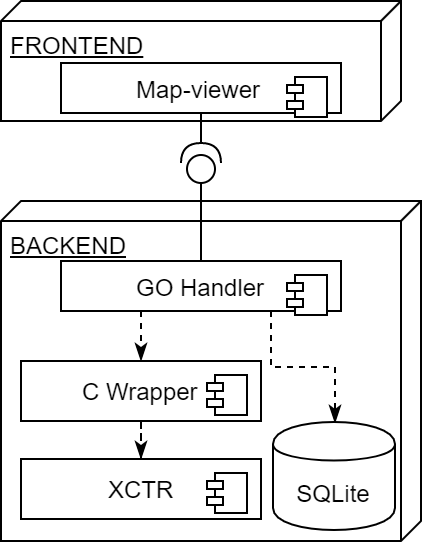
\includegraphics[width=0.5\textwidth]{figures/tview.png}}
		\end{center}
		\caption{Technical architecture of Trippy.}
		\label{fig:arch:real}
	\end{figure}
	
	The backend is implemented in the Go language, and provides a uniform API to query the information sources. This is accessed by our GIS frontend (top of Figure~\ref{fig:arch:real}), which is in charge of displaying the transport network on a web map and allows the final user to make queries by interacting with the elements of the map and its controls.

    Further details about the elements included in both the backend and the frontend of Trippy\ are discussed below.
    
    \subsubsection{\bf Representing the transport network (SQLite).}
    Since we aim at visualizing the elements of the network over a map, we need information regarding the stops and lines of the transport network, following closely the model from Figure~\ref{fig:er}. For each physical stop, along with the GPS coordinates of its location, we store a unique numeric identifier. Regarding the lines of the transport network, we basically keep the sequence of stops each line traverses. Note that, unlike the abstractions used by most public transportation networks, we consider lines to be one-way (i.e. they have a unique direction), and consequently the reversed/returning path is treated as a different line.
    
    As indicated above, we have chosen  a SQLite database to represent the network because it is conveniently portable and efficient for such small datasets. While no spatial database technology was required to deal with the GPS coordinates of the  stops, we have opted to integrate the  SpatiaLite extension\footnote{\url{https://www.gaia-gis.it/fossil/libspatialite/index}} to support storing the shapes of our lines.
    
    \subsubsection{\bf GO handler.}
    This component has two main parts. On one hand, it implements a {\em REST API} that is used to obtain the collection of stops and lines in GeoJSON format. On the other hand, it also provides a querying interface for \gls{xctr}. While the query functions themselves are implemented in \gls{xctr} using {\em C++}, we have opted for {\em Go} as our main backend language because it is specifically oriented for web services and can be easily integrated with {\em C} code. In our case, we have implemented a thin {\em C wrapper} that interacts with the \gls{xctr} libraries to load \gls{xctr} structures (when the application is launched it loads the \gls{xctr}-based representation of the trips into memory) and handle calls to the query functions.
    
    \subsubsection{\bf Map viewer.}
    The Map viewer in Trippy makes up the user interface. It is in charge of visualizing the elements of the network, and handles users’ interaction. Apart from typical functions to move around a map (i.e. zoom in/out, span, etc.), the user can interact with the elements within the map (e.g. a stop or a set of stops within a region) and access functions related to them. Those functions are supported by our backend.
    
    The Map viewer was built with a web map using the {\em Leaflet} library. With this library, it is simple to make an interactive map consisting of several interchangeable \gls{tms} and vector layers, and also to efficiently represent thousands of points or other vector-type elements.
    For additional controls, communication with the backend, state synchronization among our implemented controls and the map, we have used Vue.js\footnote{\url{https://vuejs.org}}, which is a popular web framework based on components.

	
	\section{API}
	\label{sec:api}
    As previously seen in Section~\ref{sec:newctr:algo:analysis}, by basing our interface on \gls{xctr} we are able to solve a broad range of transport-related queries, including but not limiting to:

    \begin{itemize}
    %\item[\textbf{Transport Load Queries}]
    %\item How many passengers boarded or alighted on a particular stop?
    \item How many passengers boarded or alighted on a particular stop during a specific time interval (e.g. this evening, yesterday)?
    %\item How many passengers were on a given bus in a particular moment?
    %\item At what time is a specific stop more crowded?
    %\item[\textbf{Travel Pattern Queries}]
    \item How frequently is a stop X used to switch lines during rush hours?
    \item How many passengers started/ended their trips at a specific stop X?
    \item How many passengers started their trips at stop X and ended them at stop Y during a given time interval?
    \item How many travelers had to switch lines to get to their destination during a given time interval?
    \item How many times a line is used as a start or end of a trip? Alternatively, how many times is the line used to switch between two other lines, but not as an origin nor final destination?
    %\item Calculate the arithmetic mean \ojo{llenar con algo verídico}
    \end{itemize}
    
    Along with these basic queries supported originally by \gls{xctr}, in this work, we have extended its functionality to also support a range of more complex queries that were  solved as a combination of the previous ones:
    
    \begin{itemize}
        \item How many passengers traveled from area A to area B during a time interval? 
        \item At what time is a specific stop more crowded?
        \item At what time does a line get more crowded?
        %\item What extent of the city can be reached within one hour from a certain residential area during the morning rush hour?
    \end{itemize}
    
    To support these queries, we have developed API Endpoints that we are going to discuss in the rest of this section. Note that a single request will frequently be responsible for more than one kind of query, as we it is often more practical and efficient to perform multiple types queries over the same element in \gls{xctr} for one single API request.
    
    \subsection{Stops endpoint}
    This endpoint is implemented as an {\em HTTP GET} request with the format \texttt{/stop/X}, where \texttt{X} corresponds to the queried stop identifier. This request returns the following information of the stop \texttt{X}:
    
    \begin{itemize}
        %\item The name of the stop.
        %\item The identifiers of the lines this stop belongs to.
        \item Number of passengers that had boarded.
        \item Number of times the stop was used to start a trip.
        \item Number of times the stop was used to end a trip.
    \end{itemize}
    
    Additionally, this request accepts parameters to restrict the \textit{line identifier}, \textit{lower time limit} and \textit{upper time limit}, which will filter the numerical results mentioned above.
    
    When this endpoint is queried with no parameters (\texttt{/stop/}), it will return the list of all the stops in the network, which is needed to display them on a map and initialize the interface components. Consequently, the information for each stop returned by this query will consist of the following fields:
    
    \begin{itemize}
        \item Identifier.
        \item Name of the stop.
        \item Identifiers of the lines this stop belongs to.
        \item Geographical coordinates of the location of the stop.
    \end{itemize}
    
    \subsection{Lines endpoint}
    As with stops, there also exists a line endpoint that accepts {\em HTTP GET} requests of \texttt{/line/X}, being \texttt{X} the identifier of a line. The information returned is also the equivalent of the one returned by the stop endpoint, but concerning a whole line instead of a single stop:
    
    \begin{itemize}
        \item Number of passengers that had boarded (and alighted).
        \item Number of times the line was used to start a trip.
        \item Number of times the line was used to end a trip.
    \end{itemize}
    
    This endpoint accepts filtering by a time interval with the parameters of \textit{upper and lower time limits}.
    
    There is also the listing request \texttt{/line/}, to obtain a list of existing lines with the following fields:
    
    \begin{itemize}
        \item Identifier.
        \item Name of the line.
        \item Identifiers of the stops this line contains, in order.
        \item If exists, the path of the line, encoded as a sequence of coordinates.\footnote{This information is optional, without it a line on the map can be displayed by simply connecting points with a straight line (which may not follow any road or track) or using an existing \gls{tms} layer with lines.}
    \end{itemize}
    
    \subsection{Trips endpoint}
    This endpoint is dedicated to return one single field: the number of trips that have started at any of the stops from \texttt{X$^*$} to finally end at any stop from \texttt{Y$^*$}, where both \texttt{X$^*$} and \texttt{Y$^*$} can be either a single stop or a collection of them. Due to technical reasons\footnote{The requests my contain thousands of stops, surpassing the length limits of {\em GET} requests in many web servers, proxies and even browsers.}, this requests are implemented using the {\em POST} method over the \texttt{/trip} endpoint.
    
    Both \texttt{X$^*$} and \texttt{Y$^*$} can be restricted by a \textit{line} parameter (one line for starting stops and another for ending) and also \textit{lower and upper times} (starting or ending times of the trip contained within the limits). These requests can be noticeably slow when the number of queried stops is very high (in the order of thousands).
    
    \subsection{Histograms endpoints}
    These are two endpoints that handle {\em HTTP GET} requests about time series of boarding events either for a stop (\texttt{/hstop/X}) or a line (\texttt{/hline/X}). The returned data is a sequence of pairs $<t,n>$, where $t$ is a timestamp and $n$ is the number of boardings for that timestamp.
    
    There request may be bound to a time window (by specifying \textit{lower and upper time limits}, as in the other endpoints) and also accepts an additional parameter of \textit{sampling} that, if present, will group the number boardings by a set number of seconds $s$ into bins, each time $t$ delimiting the start of a new bin that will correspond to the period $[t..t+s)$. A reasonably large sampling parameter may not only save bandwidth as less information needs to be transmitted, but also speed up the request.\footnote{In \gls{xctr}, a large sampling value may translate into more than one journey code for a line, thus making it possible to return a result before reaching the last level of the \texttt{WMJ} in the $\cnt$ operation.}
	
	\section{User Interface}
	\label{sec:ui}
	Based on the API developed from Section~\ref{sec:api}, we have developed a prototype of an accessible and intuitive user interface, based on web application technologies. In the rest of this section, we are going to demonstrate the elements of this interface in what may be read as a user manual.
	
    The interface of Trippy consists of a map as shown in Figure~\ref{fig:ui:overall}, where have set up a study case with the same bus networks from Madrid used in Section~\ref{sec:newctr:exp:data}. Every bus stop is represented by a stop and we are using the underlying Thunderforest\footnote{\url{https://www.thunderforest.com}} \gls{tms} layer to display the bus lines that connect them. Additionally, the interface presents stop selectors \textcircled{1}, line selectors \textcircled{2} and also date \textcircled{3} and time \textcircled{4} filters that allow a user to query the \gls{xctr} for information.
    
    \begin{figure}[ht]
		\begin{center}
			{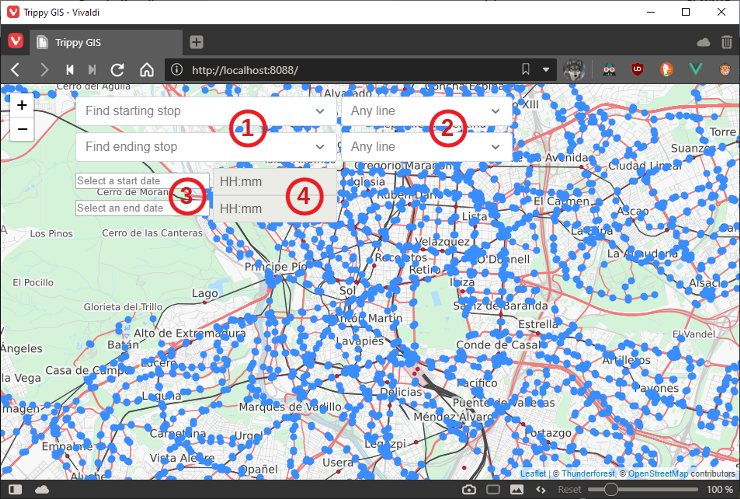
\includegraphics[width=0.9\textwidth]{screens/overall.png}}
		\end{center}
		\caption{Overall interface of Trippy.}
		\label{fig:ui:overall}
	\end{figure}
	
	As the interface shown is still in a prototype phase, it does not yet incorporate all the planned features. Concretely, we are not yet displaying the geometries of the lines nor making them interactive, and there is yet no way to make requests over the line or histogram endpoints from the previous Section~\ref{sec:api} using the graphic interface. However, we consider it complete enough to be representative of the utility that such an interface can have when powered by \gls{xctr}.
	
	By clicking on a stop, a popup is revealed with the stop name, the lines that the stop belongs to, and also the number of users that used that stop for boarding, starting or ending a trip or as a switch stop,\footnote{The number of boardings must be equal to the number of starts added to the number of switches.} as shown in Figure~\ref{fig:ui:stop} (left). These usage numbers will only be considered within the time window specified by the filter, if any. It is also possible to open a context menu for the stop with a right click, as done in Figure~\ref{fig:ui:stop} (right), and is one of the ways to specify a starting or ending stop for an X to Y query (from the trip endpoint).
	
	A future feature is planned to query the line endpoint in a similar way, in order to display usage statistics for a whole line instead of single stops. Since several line paths may overlap each other, the interface must provide a way to disambiguate the selection. The navigation among stops and lines may also be helped by providing links in the corresponding popups.
	
	%In addition, we have spatial/temporal filters allow the user to refine the displayed data, filtering by stops or time and one additional filter enables the user to refine results by line. The {\em filtering-by-stop} area allows to restrict queries to a given starting or ending stop (we can either look for their name in the filtering boxes or select them within the map). Besides, we can also provide a {\em filtering-by-datetime} which restricts also those queries to the specified starting and ending timestamps. For example, in Figure~\ref{fig:trippyIntDesc} we are querying the number of users that ``{\em boarded into a vehicle; switched-line; started a trip; ended a trip}" at the stop named {\em ``Juan de Toledo - Estaci\'on de buses"} from {\em `2019-03-12@16:00h'} to {\em `2019-03-13@16:00h'} searching on any line going through this point.
	
	\begin{figure}[ht]
		\begin{center}
			{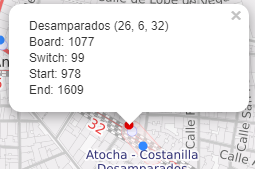
\includegraphics[width=0.49\textwidth]{screens/stop_fix.png}}
			{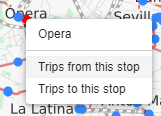
\includegraphics[width=0.49\textwidth]{screens/rclick_cut.png}}
		\end{center}
		\caption{Stop popup showing the information and usage of a single stop (left), as well as its context menu (right).}
		\label{fig:ui:stop}
	\end{figure}
	
	In the upper part of the screen we include stop and line selectors, which are implemented as custom dropdown components with a search field, as exposed in Figure~\ref{fig:ui:select}, where on the left we are looking for stops containing \textit{Bilbao} in their names, and on the right we are checking lines from \textit{Legan\'es}, from the partial query \textit{legan}.
	
	\begin{figure}[ht]
		\begin{center}
			{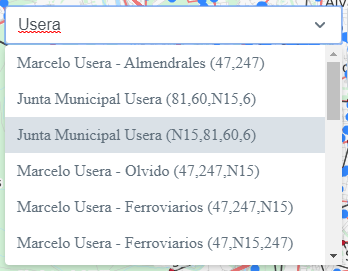
\includegraphics[width=0.49\textwidth]{screens/stop-select_cut.png}}
			{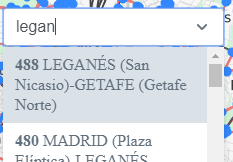
\includegraphics[width=0.49\textwidth]{screens/lines-select_cut.png}}
		\end{center}
		\caption{The stop (left) and line (right) selectors.}
		\label{fig:ui:select}
	\end{figure}
	
	As in Madrid it is frequent to have several bus stops with the exact same name for different physical stop locations, either because it is used by different lines or by the reversed direction of the same lines (as such, they tend to be located on the opposite direction of the same street), we display the lines that each stop belongs to, in order to help distinguish between these cases. Note that in the displayed version we do not distinguish the direction of the line in the interface, although we do keep track of the directions internally, and consider the reverse direction to be a separate line. These two selectors are also correlated: selecting a stop in the starting (or ending) field will restrict the starting (or ending) line selector to only those lines that the selected stop belongs to, and vice versa.
	
	The date and time filters affect all the displayed results, and can be edited with their corresponding components from Figure~\ref{fig:ui:date}. We also ensure that the selected starting and ending dates and times do not overlap: in our example only the dates starting from \texttt{2019-03-11} are available, since that is the selected starting date. If a popup is displayed while these filters are changed, the contents of the popup are dynamically updated.
	
	\begin{figure}[ht]
		\begin{center}
			{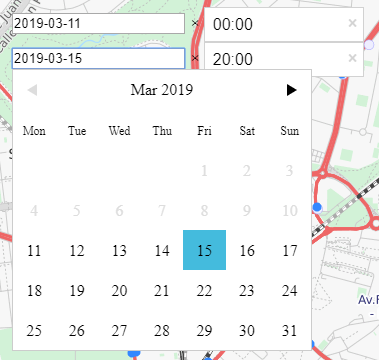
\includegraphics[width=0.5\textwidth]{screens/date_cut.png}}
		\end{center}
		\caption{The date and time filters.}
		\label{fig:ui:date}
	\end{figure}
	
	The trip endpoint (which returns number of trips performed starting with a stop X and ending with a stop Y) may be queried by either using the starting and ending stop selectors or the context menu of the stops accessible with the right click, which also fills the selected stop into the corresponding stop selector. A straight arrow will be displayed connecting the starting and the ending stops, as can be seen in Figure~\ref{fig:ui:xy}, and a popup with the total number of trips will be shown over that arrow.
	
	\begin{figure}[ht]
		\begin{center}
			{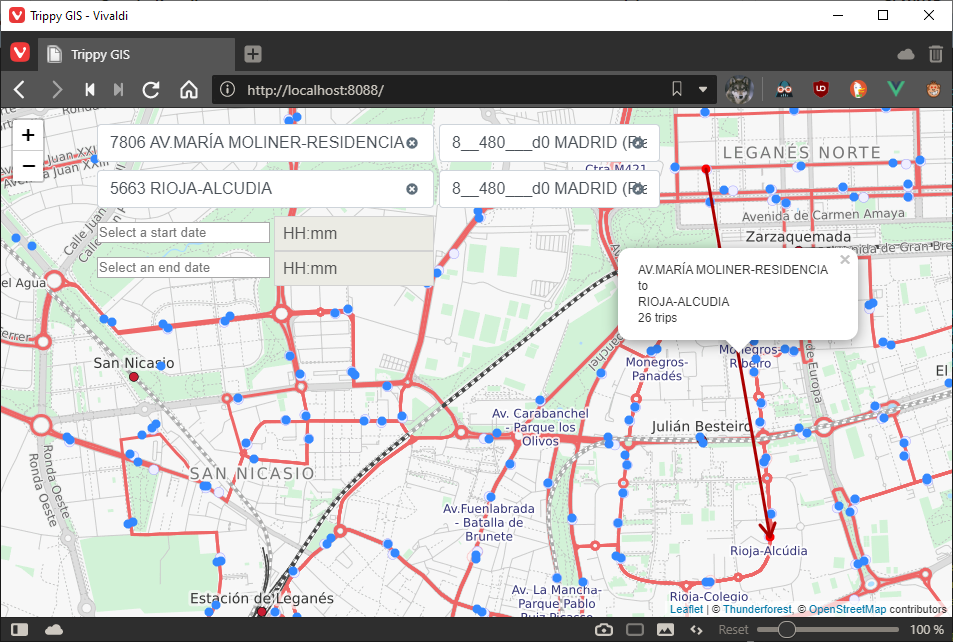
\includegraphics[width=0.9\textwidth]{screens/xy.png}}
		\end{center}
		\caption{Querying for the number of displacements between a starting and an ending stop.}
		\label{fig:ui:xy}
	\end{figure}
	
	Additionally, we allow both of these stops be be filtered by line, and the results filtered by a time window. These controls may be interacted with while the popup is open, and the number of results will be updated.
	
	We can also perform the generalized version of this query, and obtain the number of movements between a starting and a final areas, as done in Figure~\ref{fig:ui:xyarea}.
	
	\begin{figure}[ht]
		\begin{center}
			{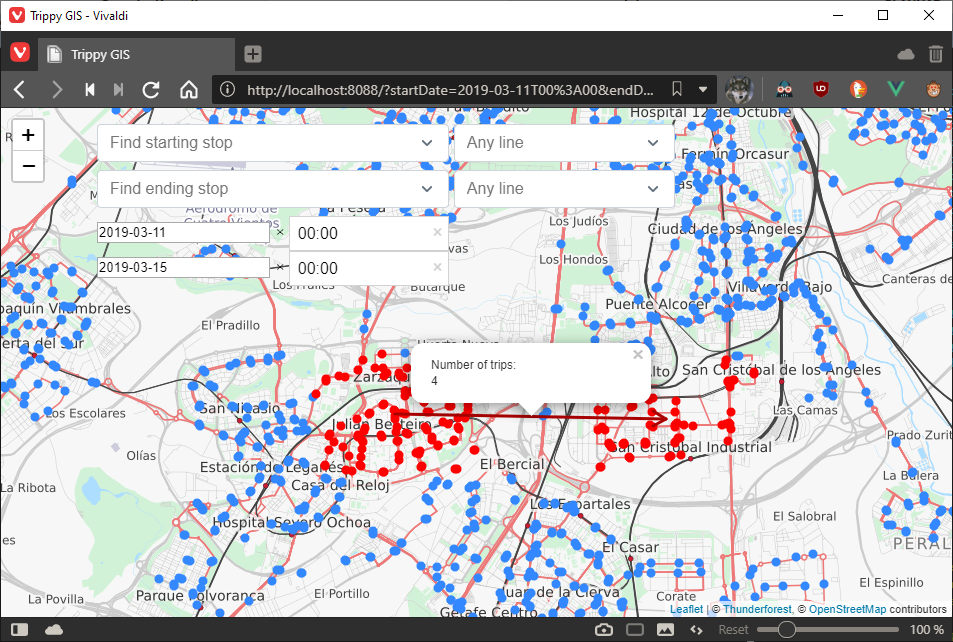
\includegraphics[width=0.9\textwidth]{screens/xy_area.png}}
		\end{center}
		\caption{Querying for the number of displacements between two areas.}
		\label{fig:ui:xyarea}
	\end{figure}
	
	In order to select the stops within a rectangular area, the user must press the  {\sc shift-key} on the keyboard and select the area of interest, by dragging the cursor. The first selected area will be considered the origin area, while the second are will be the destination. An arrow joining the two areas will appear, and a a pop-up showing the number of trips that fulfill the criteria will be displayed. Once again, this query can be refined with the time filters.
	
	While in this prototype we require the use of a keyboard to perform this query, an interactive control is planned to be able to select the starting and ending areas, with the goal of improving the accessibility of the interface.
	